%%%%%%%%%%%%%%%%%%%%%%%%%%%%%%%%%%%%%%%%%%%%%%%%%%%%%%%%%%%%%%%%
%                         My Template:                         %
%%%%%%%%%%%%%%%%%%%%%%%%%%%%%%%%%%%%%%%%%%%%%%%%%%%%%%%%%%%%%%%%

%Code(C++): \begin{lstlisting}
%Algorithm:
%\begin{breakablealgorithm}
%  \caption{?statement}
%  \begin{algorithmic}[?number]
%    \Require ?input
%    \Ensure ?output
%    \Procedure{Equal}{?parameters}
%      \State ?blabla
%    \EndProcedure
%  \end{algorithmic}
%\end{breakablealgorithm}

%Itemlisting: \begin{itemize} or \begin{enumerate}[label=(\alph*)]

%Math equation: \begin{align*}

%Table: \begin{tabular}{|c|c|c|}
%           blabla | blabla | blabla \\
%           ......
%Picture: \centerline{\includegraphics[scale=X]{FileName}

%%%%%%%%%%%%%%%%%%%%%%%%%%%%%%%%%%%%%%%%%%%%%%%%%%%%%%%%%%%%%%%%
%                         Title START!                         %
%%%%%%%%%%%%%%%%%%%%%%%%%%%%%%%%%%%%%%%%%%%%%%%%%%%%%%%%%%%%%%%%
\documentclass[11pt, a4paper, UTF8]{ctexart}
\usepackage{tikz}
\usetikzlibrary{shapes.geometric, arrows}

%%%%%%%%%%%%%%%%%%%%%%%%%%%%%%%%%%%
% File: preamble.tex
%%%%%%%%%%%%%%%%%%%%%%%%%%%%%%%%%%%
\usepackage{geometry}
\geometry{left = 1cm, right = 1cm, top = 1.5cm, bottom = 1.5cm}

\ProvidesPackage{zhfontcfg}
\usepackage{fontspec,xunicode}
\usepackage{xeCJK}
\usepackage{CJKutf8}
\usepackage{enumerate}
\defaultfontfeatures{Mapping=tex-text}
\XeTeXlinebreaklocale "zh"
\XeTeXlinebreakskip = 0pt plus 1pt minus 0.1pt
% Set fonts commands
% \newcommand\fontnamehei{文泉驿正黑}
% \newcommand\fontnamesong{文鼎PL新宋}
% \newcommand\fontnamekai{AR PL UKai CN}
% \newcommand\fontnamemono{Bitstream Vera Sans Mono}
% \newcommand\fontnameroman{Bitstream Vera Serif}
% \newcommand{\song}{\fontnamesong}
% \newcommand{\hei}{\fontnamehei}
% \newfontinstance\KAI {\fontnamekai}
% \newcommand{\kai}{\fontnamekai}
% \newCJKfontfamily\kai{FandolKai-Regular.otf}
% \newCJKfontfamily\hei{FandolHei-Regular.otf}
% \newCJKfontfamily\song{FandolSong-Regular.otf}
% \newCJKfontfamily\fang{FandolFang-Regular.otf}
% \setCJKfamilyfont{song}[BoldFont=FandolSong-Bold.otf]{FandolSong-Regular.otf}
% \setCJKfamilyfont{hei}{FandolHei-Regular.otf}
% \setCJKfamilyfont{kai}{FandolKai-Regular.otf}
\newcommand{\song}{\CJKfamily{song}}
\newcommand{\hei}{\CJKfamily{hei}}
\newcommand{\kai}{\CJKfamily{kai}}
\newcommand{\fs}{\CJKfamily{fs}}
\newcommand{\tqs}{\textquotesingle}

\defaultfontfeatures{
    Path = /usr/local/texlive/2018/texmf-dist/fonts/opentype/public/fontawesome/ }
\usepackage{fontawesome}
\newcommand{\me}[2]{\author{{\bfseries 姓名:}\underline{#1}\hspace{2em}{\bfseries 学号:}\underline{#2}}}

% Always keep this.
\newcommand{\noplagiarism}{
    \begin{center}
        \fbox{\begin{tabular}{@{}c@{}}
            请独立完成作业,不得抄袭。\\
            若参考了其它资料,请给出引用。\\
            鼓励讨论,但需独立书写解题过程。
        \end{tabular}}
    \end{center}
}

% Each hw consists of three parts:
% (1) this homework
\newcommand{\beginthishw}{\part{作业\faTasks}}
% (2) corrections (Optional)
\newcommand{\begincorrection}{\part{订正\faRefresh}}
% (3) any feedback (Optional)
\newcommand{\beginfb}{\part{反馈\faShareSquareO}}

% For math
\usepackage{amsmath}
\usepackage{amsfonts}
\usepackage{amssymb}
\usepackage{graphicx}
\usepackage{listings}
\usepackage{xcolor}
\usepackage{clrscode3e}
\usepackage{enumitem}
\usepackage{tikz}
\usepackage{tabularx}
\usepackage{multirow}
\newcolumntype{Y}{>{\centering\arraybackslash}X}
\newcolumntype{P}{>{\centering\arraybackslash}p}
%bigger integrate symbol
\usepackage{exscale}
\usepackage{relsize}
\usepackage{textcomp}

% colors
\newcommand{\red}[1]{\textcolor{red}{#1}}
\newcommand{\blue}[1]{\textcolor{blue}{#1}}
\newcommand{\teal}[1]{\textcolor{teal}{#1}}

% algorithms
\usepackage[]{algorithm}
\usepackage[noend]{algpseudocode} % noend
\makeatletter
\newenvironment{breakablealgorithm}
  {% \begin{breakablealgorithm}
      \begin{center}
          \refstepcounter{algorithm}% New algorithm
          \hrule height.8pt depth0pt \kern2pt% \@fs@pre for \@fs@ruled 画线
          \renewcommand{\caption}[2][\relax]{% Make a new \caption
              {\raggedright\textbf{\ALG@name~\thealgorithm} ##2\par}%
          \ifx\relax##1\relax % #1 is \relax
          \addcontentsline{loa}{algorithm}{\protect\numberline{\thealgorithm}##2}%
          \else % #1 is not \relax
          \addcontentsline{loa}{algorithm}{\protect\numberline{\thealgorithm}##1}%
          \fi
          \kern2pt\hrule\kern2pt
          }
          }{% \end{breakablealgorithm}
              \kern2pt\hrule\relax% \@fs@post for \@fs@ruled 画线
  \end{center}
  }
\makeatother
\renewcommand{\algorithmicrequire}{\textbf{Input:}} % Use Input in the format of Algorithm
\renewcommand{\algorithmicensure}{\textbf{Output:}} % Use Output in the format of Algorithm
% See [Adjust the indentation whithin the algorithmicx-package when a line is broken](https://tex.stackexchange.com/a/68540/23098)
\newcommand{\algparbox}[1]{\parbox[t]{\dimexpr\linewidth-\algorithmicindent}{#1\strut}}
\newcommand{\hStatex}[0]{\vspace{5pt}}
\makeatletter
\newlength{\trianglerightwidth}
\settowidth{\trianglerightwidth}{$\triangleright$~}
\algnewcommand{\LineComment}[1]{\Statex \hskip\ALG@thistlm \(\triangleright\) #1}
\algnewcommand{\LineCommentCont}[1]{\Statex \hskip\ALG@thistlm%
  \parbox[t]{\dimexpr\linewidth-\ALG@thistlm}{\hangindent=\trianglerightwidth \hangafter=1 \strut$\triangleright$ #1\strut}}
\makeatother


% Define theorem-like environments
\usepackage[amsmath, thmmarks, framed]{ntheorem}
\usepackage{framed}

\theoremheaderfont{\kai\bfseries}
\theoremstyle{break}
\theorembodyfont{\song}
% \theorembodyfont{\kai}
\theoremseparator{\vspace{1mm}}
\renewcommand*\FrameCommand{{\color{gray}\vrule width 3pt \hspace{10pt}}}
\newframedtheorem{problem}{\faCheckSquareO \ Problem}

\theorempostwork{\hrule}
\newtheorem*{solution}{\faEdit \ Solution}
\newtheorem*{revision}{\faEdit \ Revision}

\theoremstyle{plain}
\newtheorem*{cause}{\faCoffee \ Cause}
\newtheorem*{remark}{\faCommentingO \ Remark}

\theoremstyle{break}
\theoremsymbol{\ensuremath{\Box}}
\newtheorem*{proof}{\faEdit \ Proof}

\renewcommand\figurename{Figure}
\renewcommand\tablename{Table}

%enumeration
\setenumerate[1]{
    itemsep=0pt,
partopsep=0pt,
parsep=\parskip,
topsep=0pt,
leftmargin=20pt
}
\setitemize[1]{
    itemsep=0pt,
partopsep=0pt,
parsep=\parskip,
topsep=0pt,
leftmargin=20pt
}
\setdescription{
    itemsep=0pt,
partopsep=0pt,
parsep=\parskip,
topsep=0pt,
leftmargin=20pt
}
\lstset{
    language={[ISO]C++},
numbers=left,
numberstyle= \tiny,
commentstyle=\color{red!50!green!50!blue!50},
rulesepcolor=\color{red!20!green!20!blue!20},
keywordstyle=\color{blue!90}\bfseries,
showstringspaces=false,
stringstyle=\ttfamily,
}

% For figures
% for fig with caption: #1: width/size; #2: fig file; #3: fig caption
\newcommand{\fig}[3]{
    \centerline{\includegraphics[scale=#1]{#2}}
    \centerline{#3}
}

% for fig without caption: #1: width/size; #2: fig file
\newcommand{\fignc}[2]{
    \centerline{\includegraphics[scale=#1]{#2}}
}



\title{Homework 3}
\me{毕秋宇}{171860624}
\date{\today}

\begin{document}
\thispagestyle{empty}
\maketitle
% \noplagiarism

%%%%%%%%%%%%%%%%%%%%%%%%%%%%%%%%%%%%%%%%%%%%%%%%%%%%%%%%%%%%%%%%
%                       Homework START!                        %
%%%%%%%%%%%%%%%%%%%%%%%%%%%%%%%%%%%%%%%%%%%%%%%%%%%%%%%%%%%%%%%%
\beginthishw
%%%%%%%%%%%%%%%%%%%%
\begin{problem}[Decision Tree I]
    \begin{enumerate}
        \item[(1)] [5pts] Assume there is a space contains three binary features $X, Y, Z$ and the objective function is $f(x, y, z) = \neg(x\ \mathrm{XOR}\ y)$. Let $H$ denotes the decision tree constructed by these three features. Please answer the following question: Is function $f$ realizable? If the answer is yes, please draw the decision tree $H$ otherwise please give the reason.
        \item[(2)] [10pts] Now we have a dataset show by Table.1:\\
            Please use Gini value as partition criterion to draw the decision tree from the dataset. When Gini value is same for two features, please follow the alphabetical order.
    \end{enumerate}
\end{problem}

%\begin{remark}

%\end{remark}

\begin{solution}
    \begin{enumerate}
        \item[(1)] The objective function $f$ is realizable.\\
            \tikzstyle{results}=[ellipse ,text centered,draw=black]
            \tikzstyle{decisions} =[rectangle, rounded corners,text centered, draw = black]
            \tikzstyle{arrow} = [-,>=stealth]
            \begin{tikzpicture}[node distance=1cm]
                %定义具体形状和相关位置
                \node[decisions](rootnode){ $X=?$ };
                \node[decisions,below of=rootnode,yshift=-0.5cm,xshift=-2cm](rhopoint){$Y=?$};
                \node[decisions,below of=rootnode,yshift=-0.5cm,xshift=2cm](touchpoint){$Y=?$};
                % \node[results,below of=rootnode,yshift=-0.5cm,xshift=2.5cm](result1){坏瓜};
                \node[results,below of=rhopoint,yshift=-0.5cm,xshift=-1cm](result2){1};
                \node[results,below of=rhopoint,yshift=-0.5cm,xshift=1cm](result3){0};
                \node[results,below of=rhopoint,yshift=-0.5cm,xshift=3cm](result4){0};
                \node[results,below of=rhopoint,yshift=-0.5cm,xshift=5cm](result5){1};
                %连接形状
                \draw [arrow] (rootnode) -- node [left,font=\small] {1} (rhopoint);
                \draw [arrow] (rootnode) -- node [right,font=\small] {0} (touchpoint);
                % \draw [arrow] (rootnode) -- node [right,font=\small] {模糊} (result1);
                \draw [arrow] (rhopoint) -- node [left,font=\small] {1} (result2);
                \draw [arrow] (rhopoint) -- node [right,font=\small] {0} (result3);
                \draw [arrow] (touchpoint) -- node [left,font=\small] {1} (result4);
                \draw [arrow] (touchpoint) -- node [right,font=\small] {0} (result5);
            \end{tikzpicture}
        \item[(2)] We know that $\mathrm{Gini}(D)=1-\sum_{k=1}^{|y|}p_{k}^{2}$, the original $\mathrm{Gini}(D)=1-\frac{1}{4}-\frac{1}{4}=\frac{1}{2}$,\\
            $\mathrm{Dini}(D,X)=\frac{4}{8}(1-\frac{1}{4}-\frac{1}{4})+\frac{4}{8}(1-\frac{1}{4}-\frac{1}{4})=\frac{1}{2}$\\
            $\mathrm{Dini}(D,Y)=\frac{4}{8}(1-\frac{1}{4}-\frac{1}{4})+\frac{4}{8}(1-\frac{1}{4}-\frac{1}{4})=\frac{1}{2}$\\
            $\mathrm{Dini}(D,Z)=\frac{6}{8}(1-\frac{4}{9}-\frac{1}{9})+\frac{2}{8}(1-1)=\frac{1}{3}$\\
            So we choose $Z$ as the first property to divide.\\
            $\mathrm{Dini}(D,X)=\frac{3}{6}(1-\frac{4}{9}-\frac{1}{9})+\frac{3}{6}(1-\frac{4}{9}-\frac{1}{9})=\frac{4}{9}$\\
            $\mathrm{Dini}(D,Y)=\frac{3}{6}(1-\frac{4}{9}-\frac{1}{9})+\frac{3}{6}(1-\frac{4}{9}-\frac{1}{9})=\frac{4}{9}$\\
            Then we choose $X$ as the second property to divide.\\
            And the dicision tree is just as follows:\\
            \tikzstyle{results}=[ellipse ,text centered,draw=black]
            \tikzstyle{decisions} =[rectangle, rounded corners,text centered, draw = black]
            \tikzstyle{arrow} = [-,>=stealth]
            \begin{tikzpicture}[node distance=1cm]
                %定义具体形状和相关位置
                \node[decisions](rootnode){ $Z=?$ };
                \node[decisions,below of=rootnode,yshift=-0.5cm,xshift=-1cm](rhopoint){$X=?$};
                \node[decisions,below of=rootnode,yshift=-2.0cm,xshift=-2cm](touchpoint1){$Y=?$};
                \node[decisions,below of=rootnode,yshift=-2.0cm,xshift=0cm](touchpoint2){$Y=?$};
                \node[results,below of=rootnode,yshift=-0.5cm,xshift=1cm](result1){0};
                \node[results,below of=rhopoint,yshift=-2.0cm,xshift=-2cm](result2){0};
                \node[results,below of=rhopoint,yshift=-2.0cm,xshift=-0.5cm](result3){1};
                \node[results,below of=rhopoint,yshift=-2.0cm,xshift=0.5cm](result4){1};
                \node[results,below of=rhopoint,yshift=-2.0cm,xshift=2.0cm](result5){0};
                %连接形状
                \draw [arrow] (rootnode) -- node [left,font=\small] {1} (rhopoint);
                \draw [arrow] (rootnode) -- node [right,font=\small] {0} (result1);
                \draw [arrow] (rhopoint) -- node [left,font=\small] {1} (touchpoint1);
                \draw [arrow] (rhopoint) -- node [left,font=\small] {0} (touchpoint2);
                \draw [arrow] (touchpoint1) -- node [left,font=\small] {0} (result2);
                \draw [arrow] (touchpoint1) -- node [left,font=\small] {1} (result3);
                \draw [arrow] (touchpoint2) -- node [left,font=\small] {1} (result4);
                \draw [arrow] (touchpoint2) -- node [left,font=\small] {0} (result5);
            \end{tikzpicture}
    \end{enumerate}
\end{solution}
%%%%%%%%%%%%%%%%%%%%%
\begin{problem}[Decision Tree]
    Consider the following matrix:
    \[\left[
        \begin{matrix}
            24 & 53 & 23 & 25 & 32 & 52 & 22 & 43 & 52 & 48\\
            40 & 52 & 25 & 77 & 48 & 110 & 38 & 44 & 27 & 65
        \end{matrix}
        \right]
    \]
    which contains 10 examples and each example contains two features $x_1$ and $x_2$ . The corresponding label of these 10 examples as follows:
    \[\left[
        \begin{matrix}
            1 & 0 & 0 & 1 & 1 & 1 & 1 & 0 & 0 & 1
        \end{matrix}
        \right]
    \]
    In this problem, we want to build a decision tree to do the classification task.
    \begin{enumerate}
        \item[(1)][5pts] Calculate the entropy of the root node.
        \item[(2)][10pts] Building your decision tree. What is your split rule and the classification error?
        \item[(3)][10pts] A multivariate decision tree is a generalization of univariate decision trees, where more than one attribute can be used in the decision for each split. That is, the split need not be orthogonal to a feature’s axis.\\
            Building a multivariate decision tree where each decision rule is a linear classifier that makes decisions based on the sign of $\alpha x_1 + \beta x_2 − 1$. What is the depth of your tree, as well as $\alpha$ and $\beta$?
    \end{enumerate}
\end{problem}

%\begin{remark}

%\end{remark}

\begin{solution}
    \begin{enumerate}
        \item[(1)] According to the definition $\mathrm{End}(D)=-\frac{3}{5}\log_{2}\frac{3}{5}-\frac{2}{5}\log_{2}\frac{3}{5}\approx 0.97095$
        \item[(2)]
            The split rule is $\mathrm{Gini}$ value, and classification error is $\frac{1}{10}$\\
            \tikzstyle{results}=[ellipse ,text centered,draw=black]
            \tikzstyle{decisions} =[rectangle, rounded corners,text centered, draw = black]
            \tikzstyle{arrow} = [-,>=stealth]
            \begin{tikzpicture}[node distance=1cm]
                %定义具体形状和相关位置
                \node[decisions](rootnode){ $x_2\leq 52?$ };
                \node[decisions,below of=rootnode,yshift=-0.5cm,xshift=-1cm](rhopoint){$x_1\geq23?$};
                \node[results,below of=rootnode,yshift=-0.5cm,xshift=1cm](result1){1};
                \node[results,below of=rhopoint,yshift=-0.5cm,xshift=-1cm](result2){0};
                \node[results,below of=rhopoint,yshift=-0.5cm,xshift=1cm](result3){1};
                % \node[results,below of=rhopoint,yshift=-0.5cm,xshift=5cm](result5){1};
                %连接形状
                \draw [arrow] (rootnode) -- node [left,font=\small] {true} (rhopoint);
                \draw [arrow] (rootnode) -- node [right,font=\small] {false} (result1);
                \draw [arrow] (rhopoint) -- node [left,font=\small] {true} (result2);
                \draw [arrow] (rhopoint) -- node [right,font=\small] {false} (result3);
            \end{tikzpicture}
        \item[(3)] The depth of my tree is 2, with $\alpha=-\frac{1}{10},\beta=\frac{1}{10}$.\\
            \tikzstyle{results}=[ellipse ,text centered,draw=black]
            \tikzstyle{decisions} =[rectangle, rounded corners,text centered, draw = black]
            \tikzstyle{arrow} = [-,>=stealth]
            \begin{tikzpicture}[node distance=1cm]
                \node[decisions](rootnode){ $-\frac{1}{10}x_1+\frac{1}{10}x_2-1\leq 0?$ };
                \node[results,below of=rootnode,yshift=-0.5cm,xshift=1cm](result1){1};
                \node[results,below of=rootnode,yshift=-0.5cm,xshift=-1cm](result2){0};
                \draw [arrow] (rootnode) -- node [right,font=\small] {false} (result1);
                \draw [arrow] (rootnode) -- node [left,font=\small] {true} (result2);
            \end{tikzpicture}
    \end{enumerate}
\end{solution}
%%%%%%%%%%%%%%%%%%%%%
\begin{problem}[Convolutional Neural Networks]
    Using Fig. 1 as an example. Assuming that the loss function of the convolutional neural network is cross-entropy:
    \begin{enumerate}
        \item[(1)][5 pts] Briefly describe the forward propagation process;
        \item[(2)][5 pts] What is the difference between Relu and Sigmoid activation functions;
        \item[(3)][5 pts] Derivation of the fully connected layer;
        \item[(4)][5 pts] Derivation of the pooling layer with average pooling;
        \item[(5)][5 pts] Derivation of the convolutional layer with Relu;
    \end{enumerate}
\end{problem}

%\begin{remark}

%\end{remark}

\begin{solution}
    \begin{enumerate}
        \item[(1)] Firstly, the input $28\times 28$ map is convoluted to be six $24\times 24$ maps, and then the pooling layer sample the convolutional six $24\times 24$ maps into six $12\times 12$ maps. Next, the new $12\times 12$ maps are convoluted to be twelve $8\times 8$ maps, and then we use pooling layer to sample the twelve $8\times 8$ maps into twelve $4\times 4$ maps. Finally, we use softmax as the output layer to show our predict.\\
            In the following table, $X$ is the input of each layer, $Y$ is the output and $\sigma$ is the avtivation function $\beta$ is the pooling function.
            \begin{table}[H]
                \begin{center}
                    \begin{tabular}{|l|l|l|}
                        \hline
                        Layer & Parameters & Output \\ \hline
                        Input & None & $1*Y(28*28)$ \\ \hline
                        Convolutional Layer1 & $X=Y(28*28)~~Y=\sigma(W*X+b)$ & $6*Y(24*24)$\\ \hline
                        Pooling Layer1 & $X=Y(24*24)~~Y=\beta(X)+b$ & $6*Y(12*12)$\\ \hline
                        Convolutional Layer2 & $X=Y(12*12)~~Y=\sigma(W*X+b)$ & $12*Y(8*8)$\\ \hline
                        Pooling Layer2 & $X=Y(5*5)~~Y=\beta(X)+b$ & $12*Y(4*4)$\\ \hline
                        Output & $X=Y(4*4)~~Y=(W*X+b)$& $1*Y(12)$\\ \hline
                    \end{tabular}
                \end{center}
            \end{table}
        \item[(2)] sigmoid function is in the form of $f(x)=\frac{1}{1+e^{-x}}$ and relu is in the form of $f(x)=\max(0,x)$. And we know that sigmoid function is smooth that is to say sigmoid function is everywhere can get derivation, however relu function doesn't have derivation when $x=0$.
        \item[(3)] By the architecture of network, we know that in the full connected layer $Y = \mathrm{softmax}(W*X+b)$, denote $p$ as the expected output $q$ as the actual output, and the cross entropy $H(p,q)=-\sum_{x}p(x)\log q(x)$. So we get that:
            \[\frac{\partial H}{\partial w}=\frac{\partial H}{\partial q(x)}\frac{\partial q(x)}{\partial p(x)}\frac{\partial p(x)}{\partial w}\]
            We get that
            \[\frac{\partial H}{\partial q(x)}=-\frac{p(x)}{q(x)}\]
            \[\frac{\partial q(x)}{\partial p(x)}=q(x)(1-q(x))\]
            \[\frac{\partial p(x)}{\partial w}=x\]
            \[\frac{\partial p(x)}{\partial b}=1\]
            Thus
            \[\frac{\partial H}{\partial w}=(-\frac{p(x)}{q(x)})\times q(x)(1-q(x))\times x=xp(q-1)\]
            \[\frac{\partial H}{\partial b}=(-\frac{p(x)}{q(x)})\times q(x)(1-q(x))=p(q-1)\]
        \item[(4)] We denote that $x^n=W^{n}x^{n-1}+b^n$.\\
            That is to say:
            \[\frac{\partial H^{n}}{\partial W^{n}}=\sum\sum\frac{\partial H^{n}}{\partial x^{n}}\frac{\partial x^{n}}{\partial W^{n}}=\sum\sum\frac{\partial H^{n}}{\partial x^{n}}\sum\sum x^{n-1}\]
            \[\frac{\partial H^{n}}{\partial b^{n}}=\sum\sum\frac{\partial H^{n}}{\partial x^{n}}\frac{\partial x^{n}}{\partial b^{n}}=\sum\sum\frac{\partial H^{n}}{\partial x^{n}}\]
        \item[(5)] We denote that in the convolutional layer $x^{n}=\mathrm{delu}(\sum\sum\sum W^{n}_{a,b,c}x^{n}_{i,j})+b^{n}$.\\
            So we get that:
            \[\frac{\partial H^{n}}{\partial W^{n}_{a,b,c}}=\frac{\partial H^{n}}{\partial x^{n}_{i,j}}\frac{\partial x^{n}_{i,j}}{W^{n}_{a,b,c}}=\frac{\partial H^{n}}{\partial x^{n}}a^{n-1}_{i,j}\mathrm{delu}^{\prime}(a^{n-1}_{i,j})\]
            If $a^{n-1}_{i,j}<0$, then
            \[\frac{\partial H^{n}}{\partial W^{n}_{a,b,c}}=0.\]\\
            Else
            \[\frac{\partial H^{n}}{\partial W^{n}_{a,b,c}}=\frac{\partial H^{n}}{\partial x^{n}}a^{n-1}_{i,j}.\]
            And we also get
            \[\frac{\partial H^{n}}{\partial b^{n}}=\frac{\partial H^{n}}{\partial x^{n}_{i,j}}\frac{\partial x^{n}_{i,j}}{\partial b^{n}}\]
            If $a^{n-1}_{i,j}<0$, then
            \[\frac{\partial H^{n}}{\partial b^{n}}=0.\]\\
            Else
            \[\frac{\partial H^{n}}{\partial b^{n}}=\frac{\partial H^{n}}{\partial x^{n}}.\]

    \end{enumerate}
\end{solution}
%%%%%%%%%%%%%%%%%%%%%
\begin{problem}[Neural Network in Practice]
    In this task, you are asked to build a Convolutional Neural Networks (CNNs) from scratch and examine performance of the network you just build on $\textbf{MNIST}$ dataset. Fortunately, there are some out-of-the-box deep learning tools that can help you get started very quickly. For this task, we would like to ask you to work with the $\textbf{Pytorch}$ deep learning framework. Additionally, Pytorch comes with a built-in dataset class for MNIST digit classification task in the $\textbf{torchvision}$ package, including a training set and a validation set. You may find a pytorch introduction at here. Note that, you can use CPU or GPU for training at your choice.\\
    Please find the detailed requirements below.
    \begin{enumerate}
        \item[(1)][5 pts] You are encouraged to implement the code using $Python3$, implementations in any other programming language will not be judged. Please name the source file (which contains the main function) as $CNN main.py$. Finally, your code needs to print the performance on the provided validation set once executed.
        \item[(2)][10 pts] Use any type of CNNs as you want and draw graphs to show your network architecture in the submitted report. You are encouraged to try more architectures.
        \item[(3)][15 pts] During training, you may want to try some different optimization algorithms, such as SGD, Adam. Also, you need to study the effect of learning rate and the number of epoch, on the performance (accuracy).
        \item[(4)][5 pts] Plot graphs (learning curves) to demonstrate the change of training loss as well as the validation loss during training.
    \end{enumerate}
\end{problem}

%\begin{remark}

%\end{remark}

\begin{solution}
    \begin{enumerate}
        \item[(1)] The details of my relization can be seen in the code.
            % The performance of my CNN in the test set is as follows:
            % \begin{figure}[H]
            % \centering
            % 
\includegraphics[scale=0.6]{3.png}
            % % \caption{this is a figure demo}
            % % \label{fig:pathdemo}
            % \end{figure}
        \item[(2)] The architecture of my network is as follows:
            \begin{figure}[H]
                \centering
                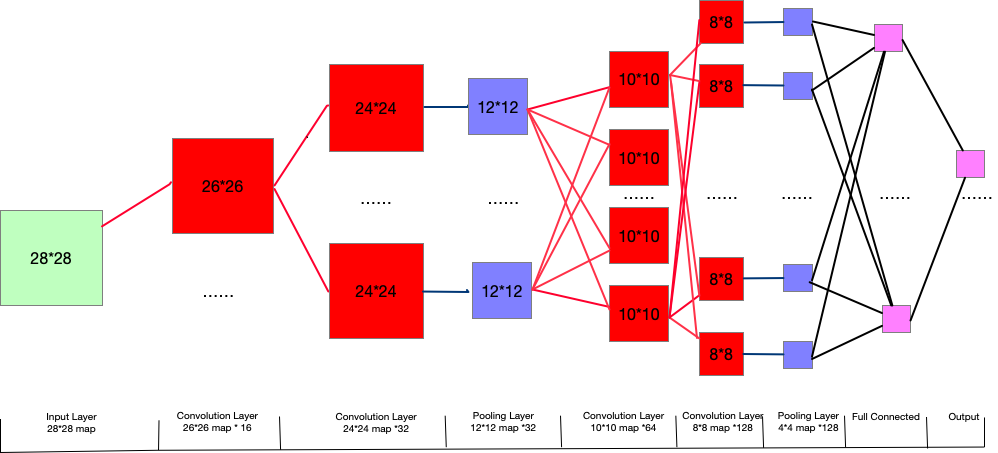
\includegraphics[scale=0.5]{1.png}
                % \caption{this is a figure demo}
                % \label{fig:pathdemo}
            \end{figure}
            \begin{figure}[H]
                \centering
                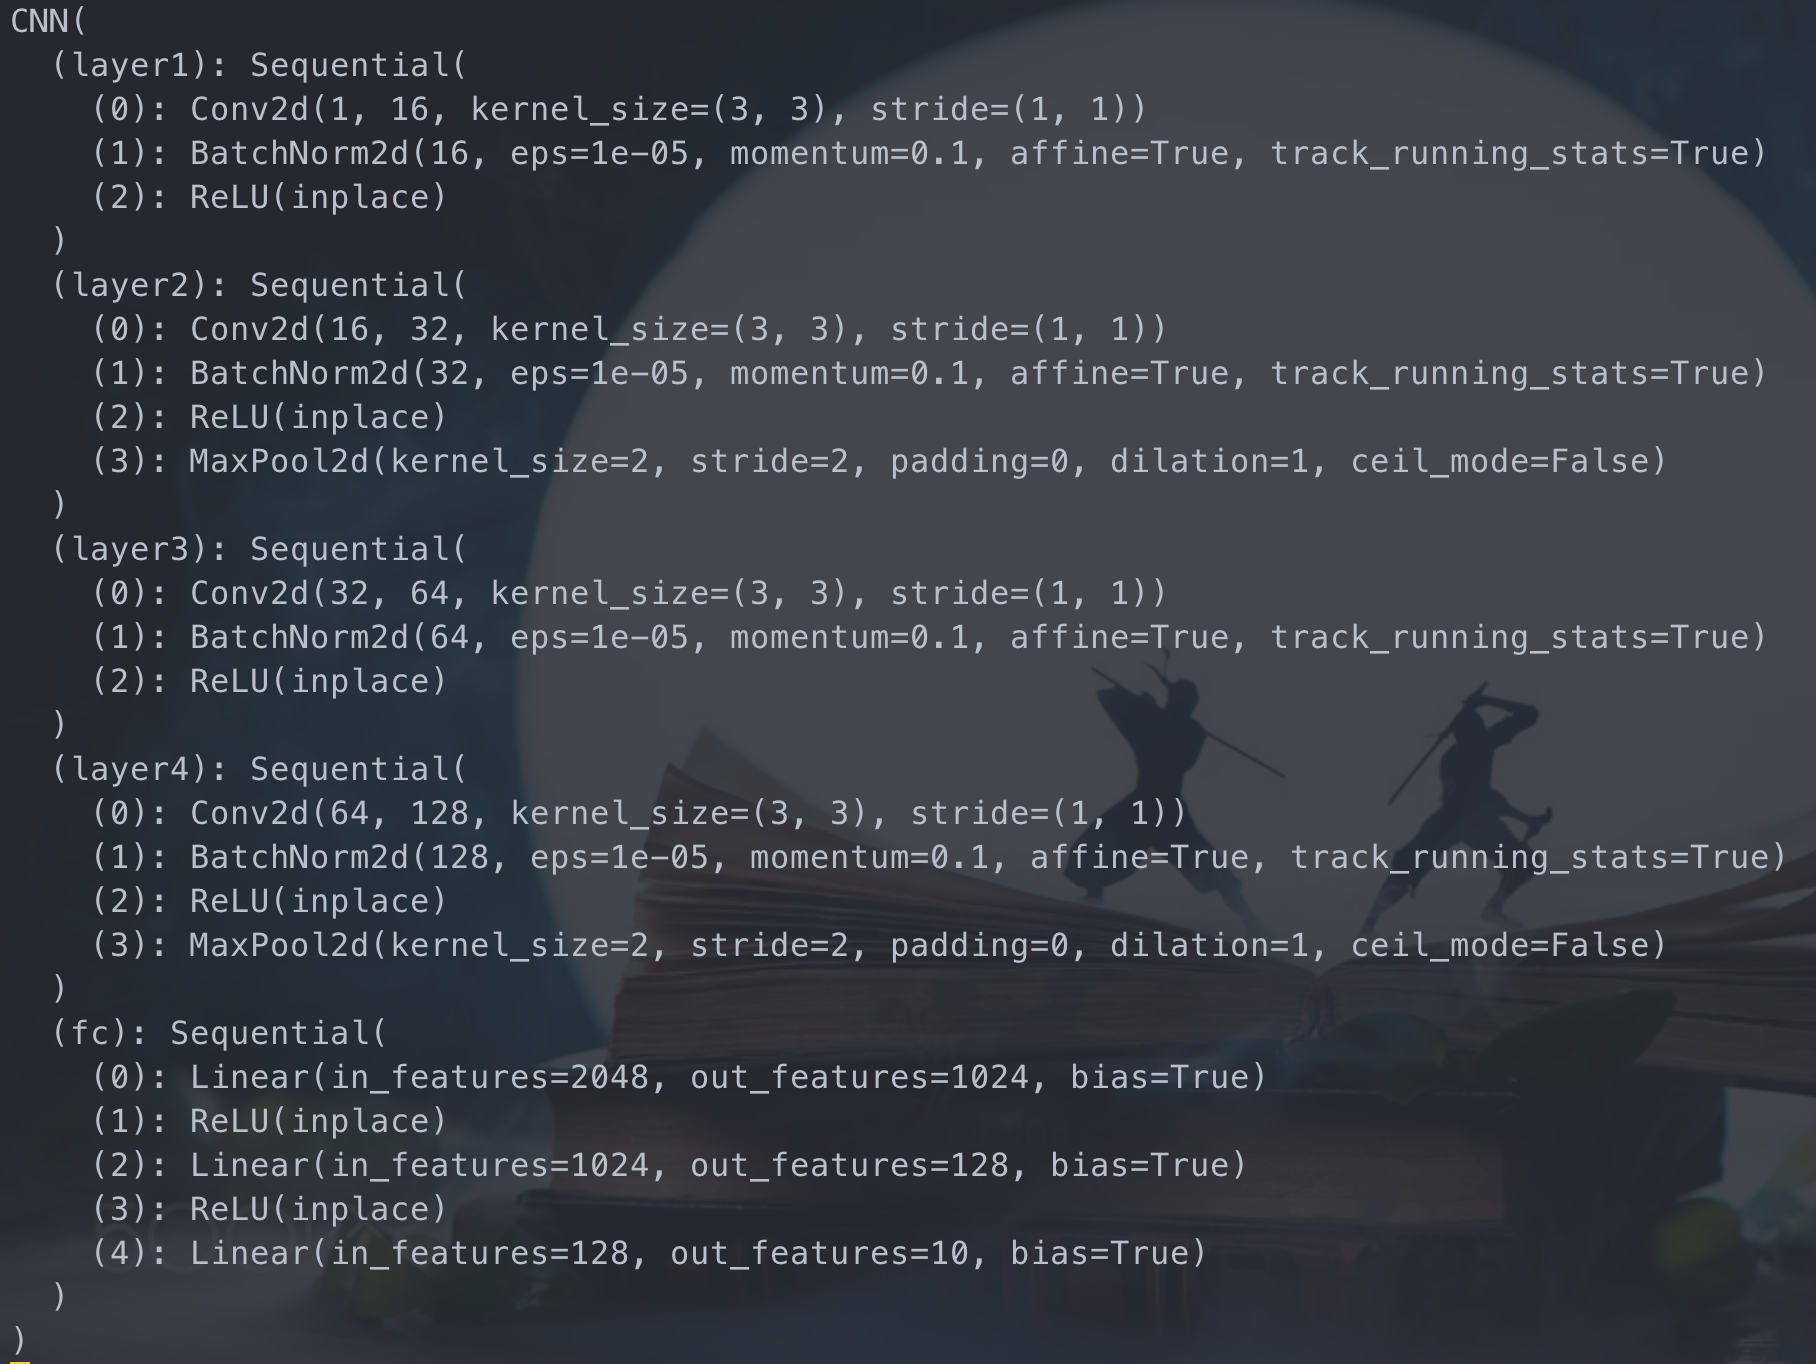
\includegraphics[scale=0.5]{5.png}
                \caption{network architecture}
                % \label{fig:pathdemo}
            \end{figure}
        \item[(3)] The change with epoch is as follows:
            \begin{figure}[H]
                \centering
                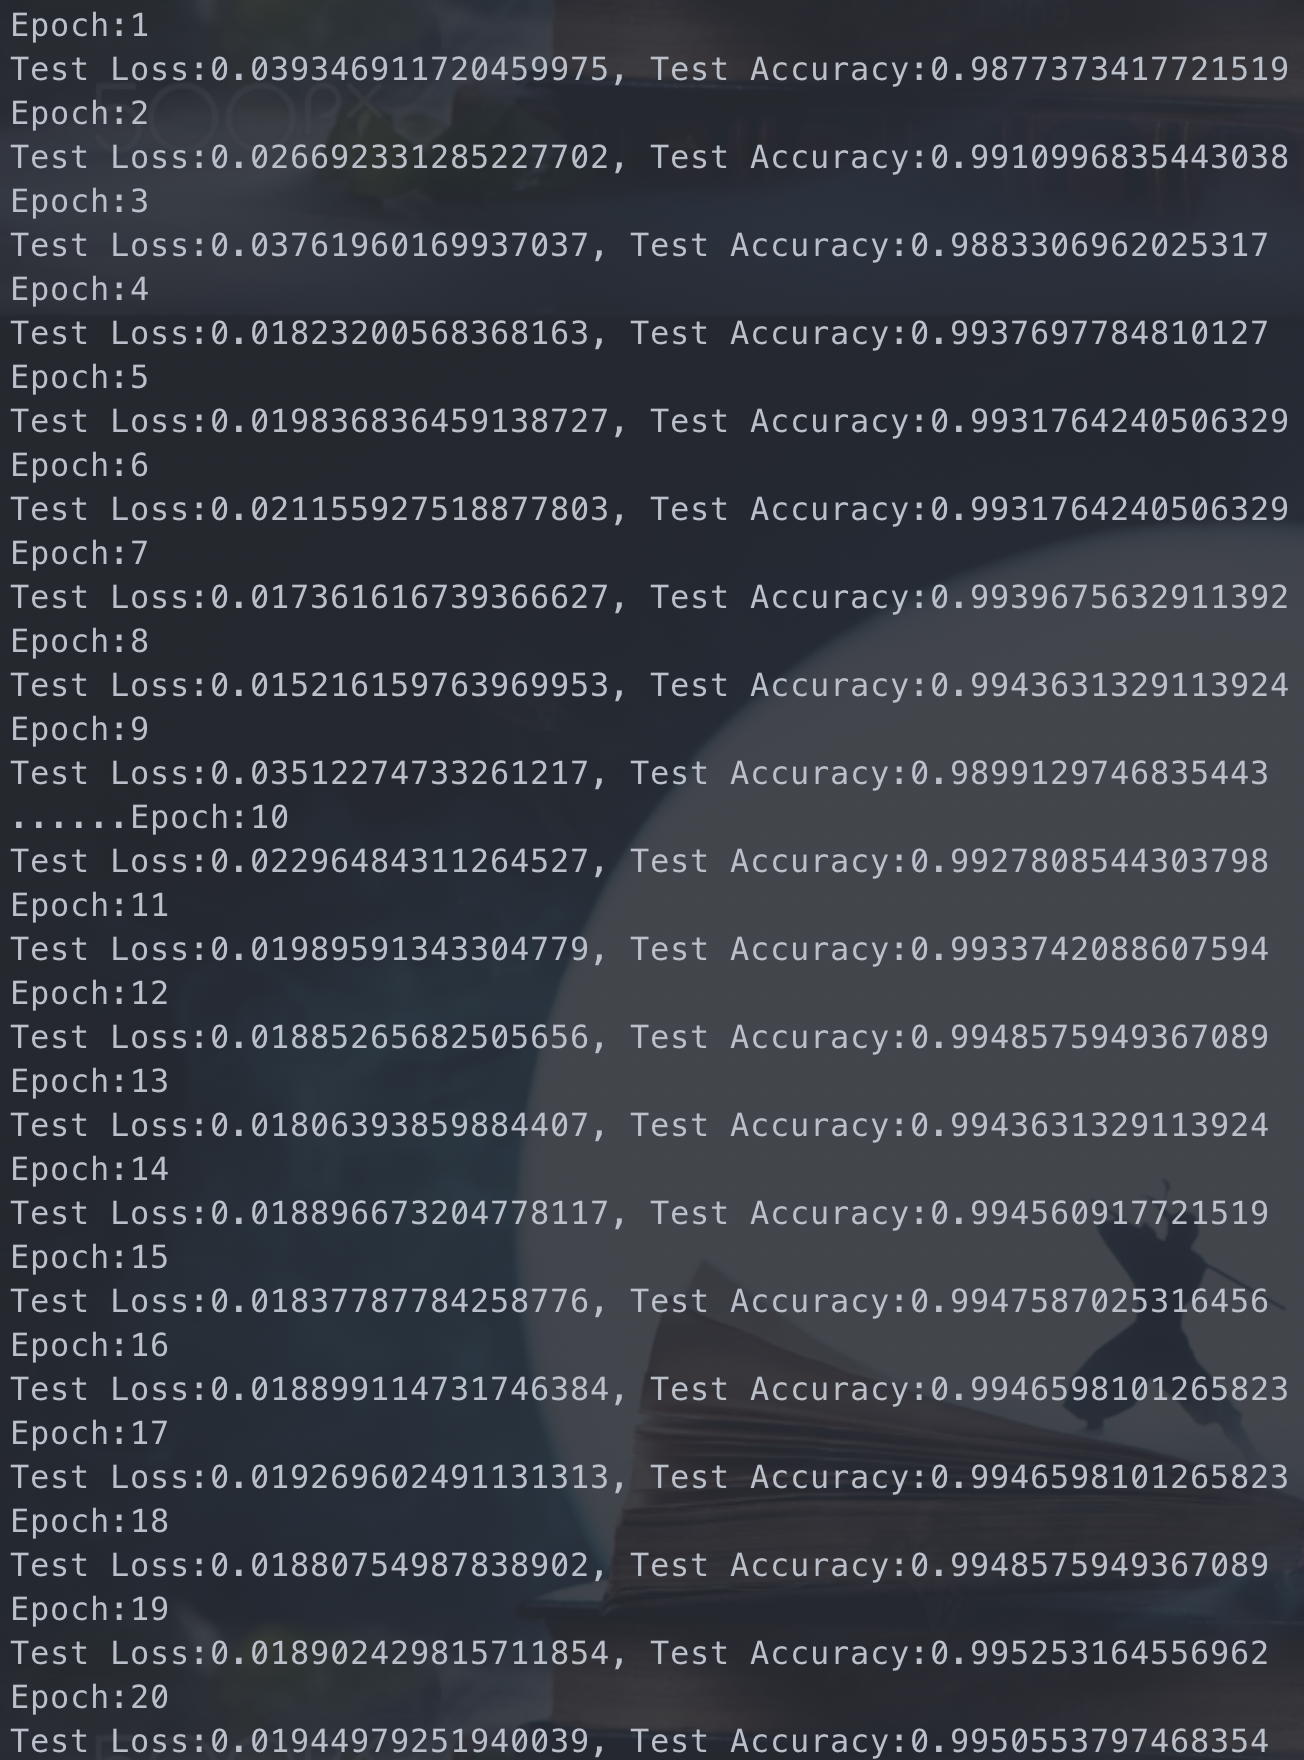
\includegraphics[scale=0.30]{8.png}
                \caption{performance}
                % \label{fig:pathdemo}
            \end{figure}
            And with different optimization algorithms the performance is as follows:
            \begin{figure}[H]
                \centering
                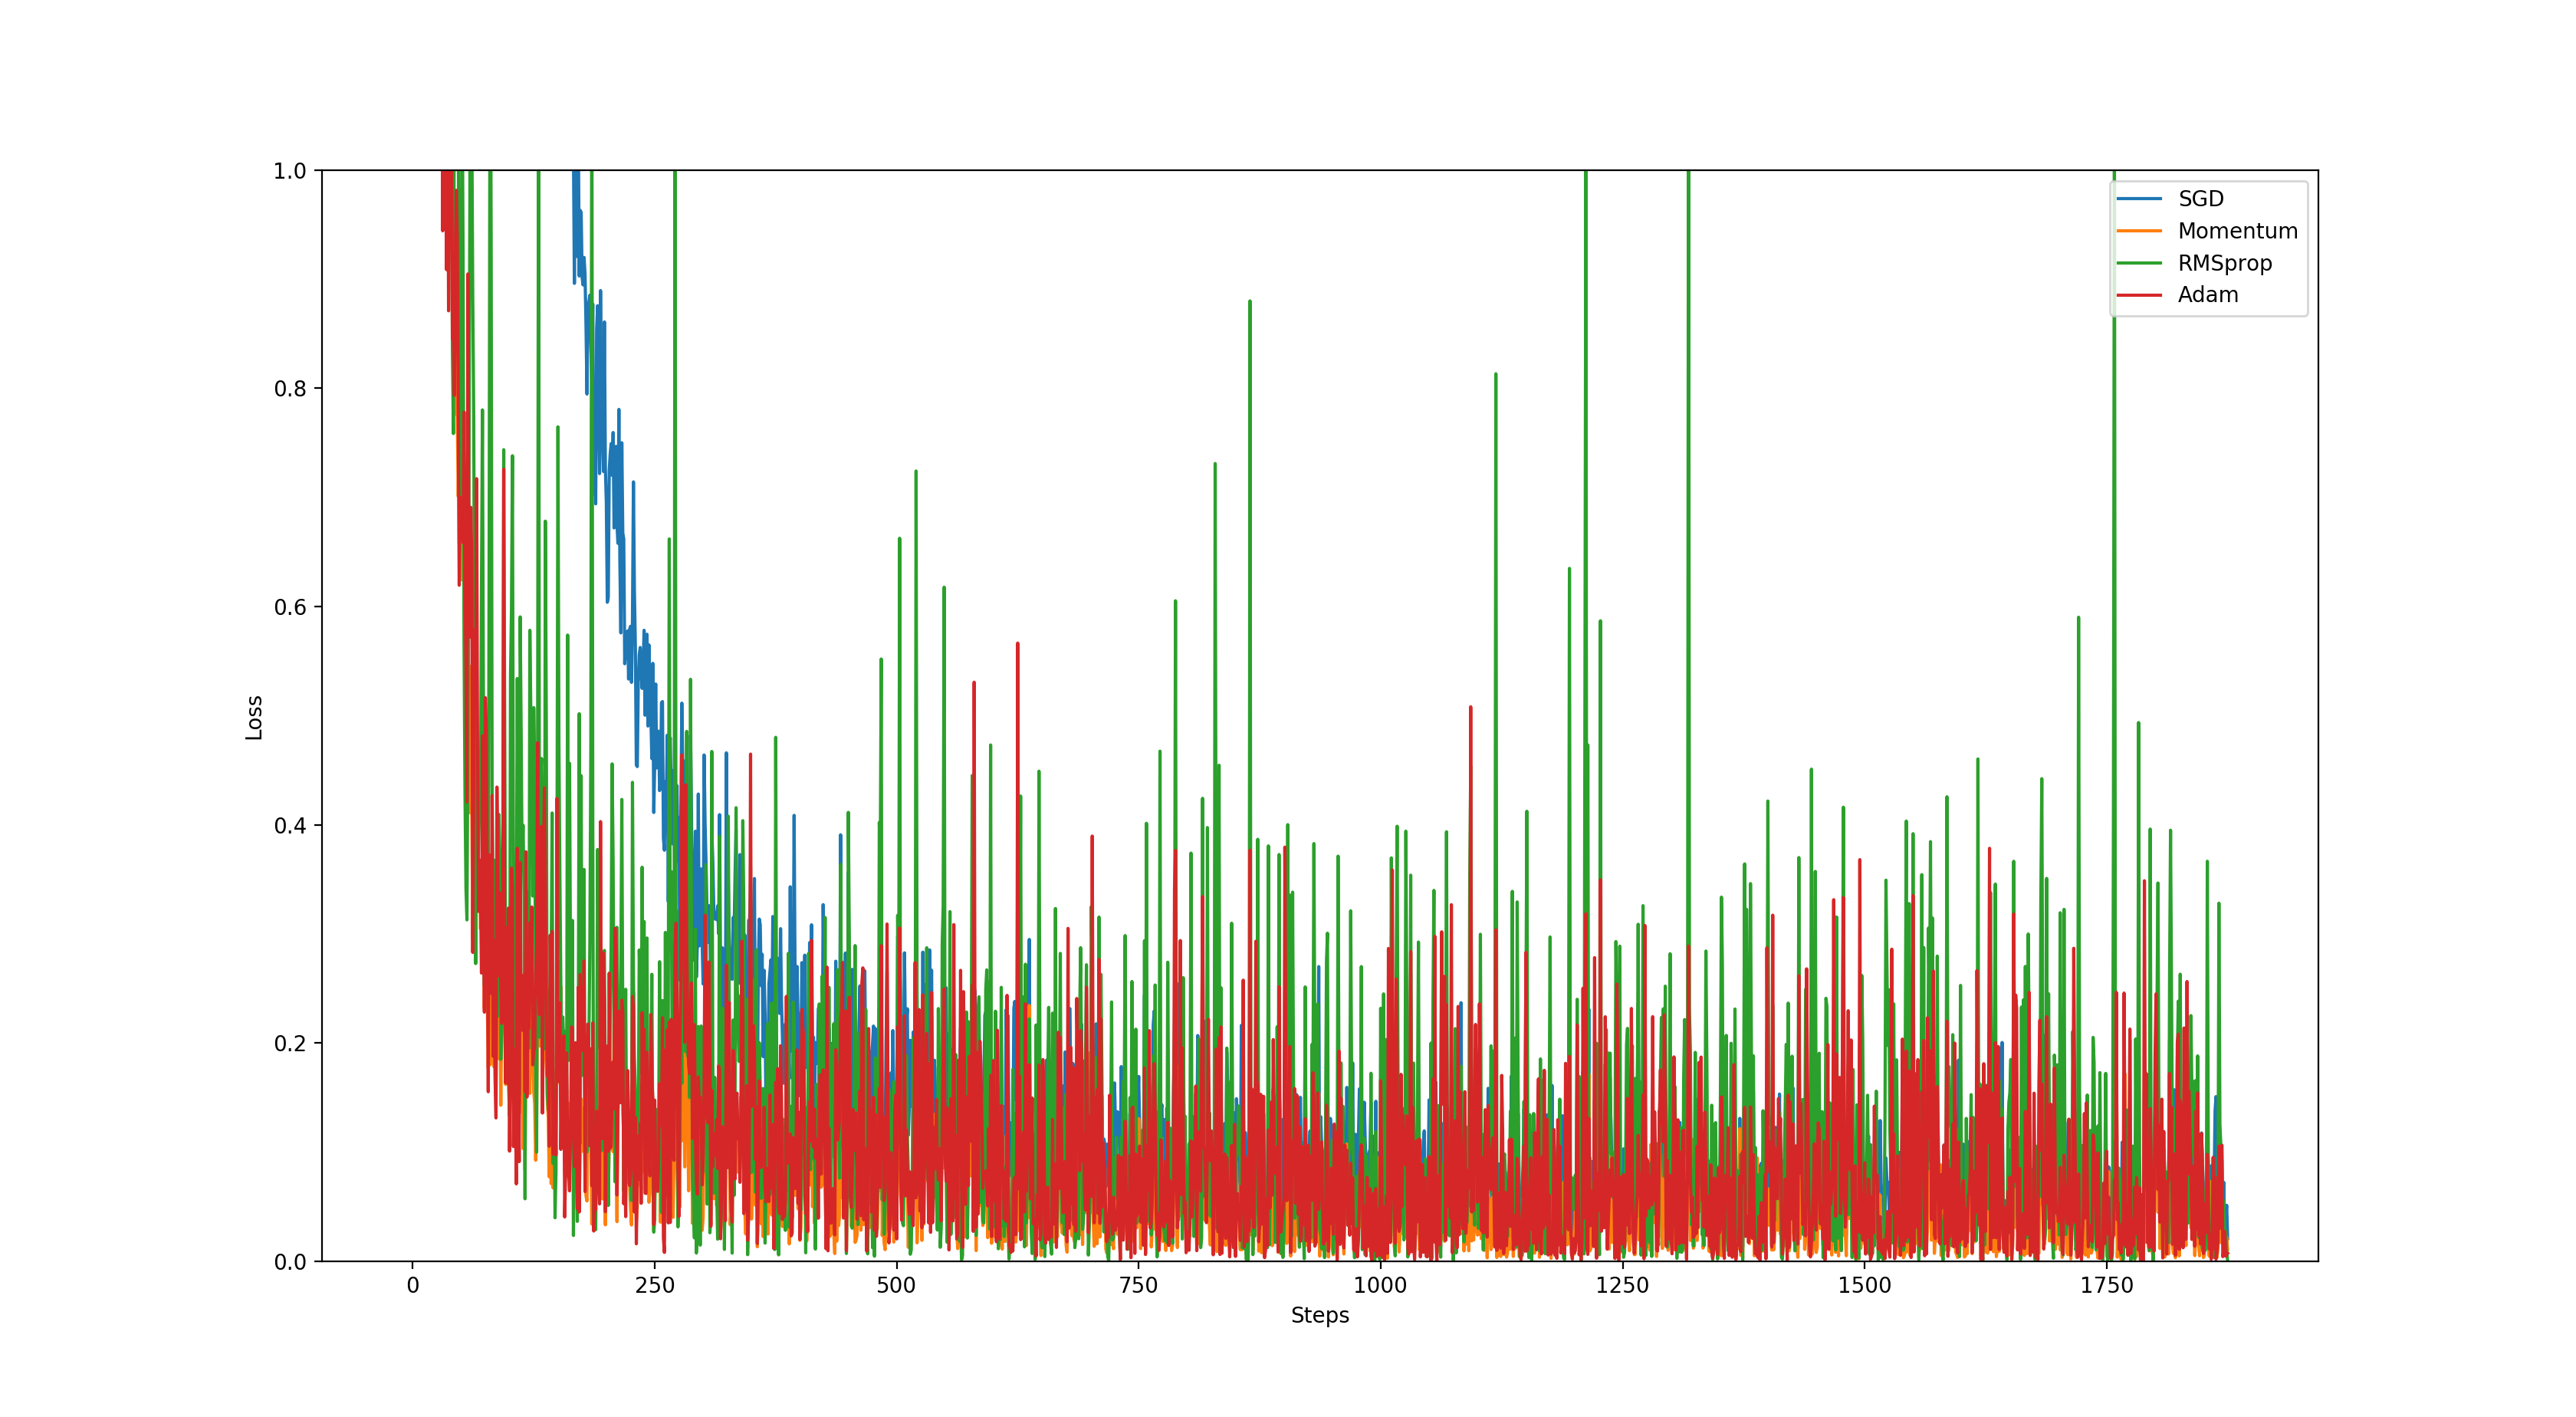
\includegraphics[scale=0.35]{4.png}
                \caption{optimization algorithms}
                % \label{fig:pathdemo}
            \end{figure}
            Then we choose SGD as the optimization and 20 epoch to create my CNN.
        \item[(4)] the curve of change of training loss is as follows:
            \begin{figure}[H]
                \centering
                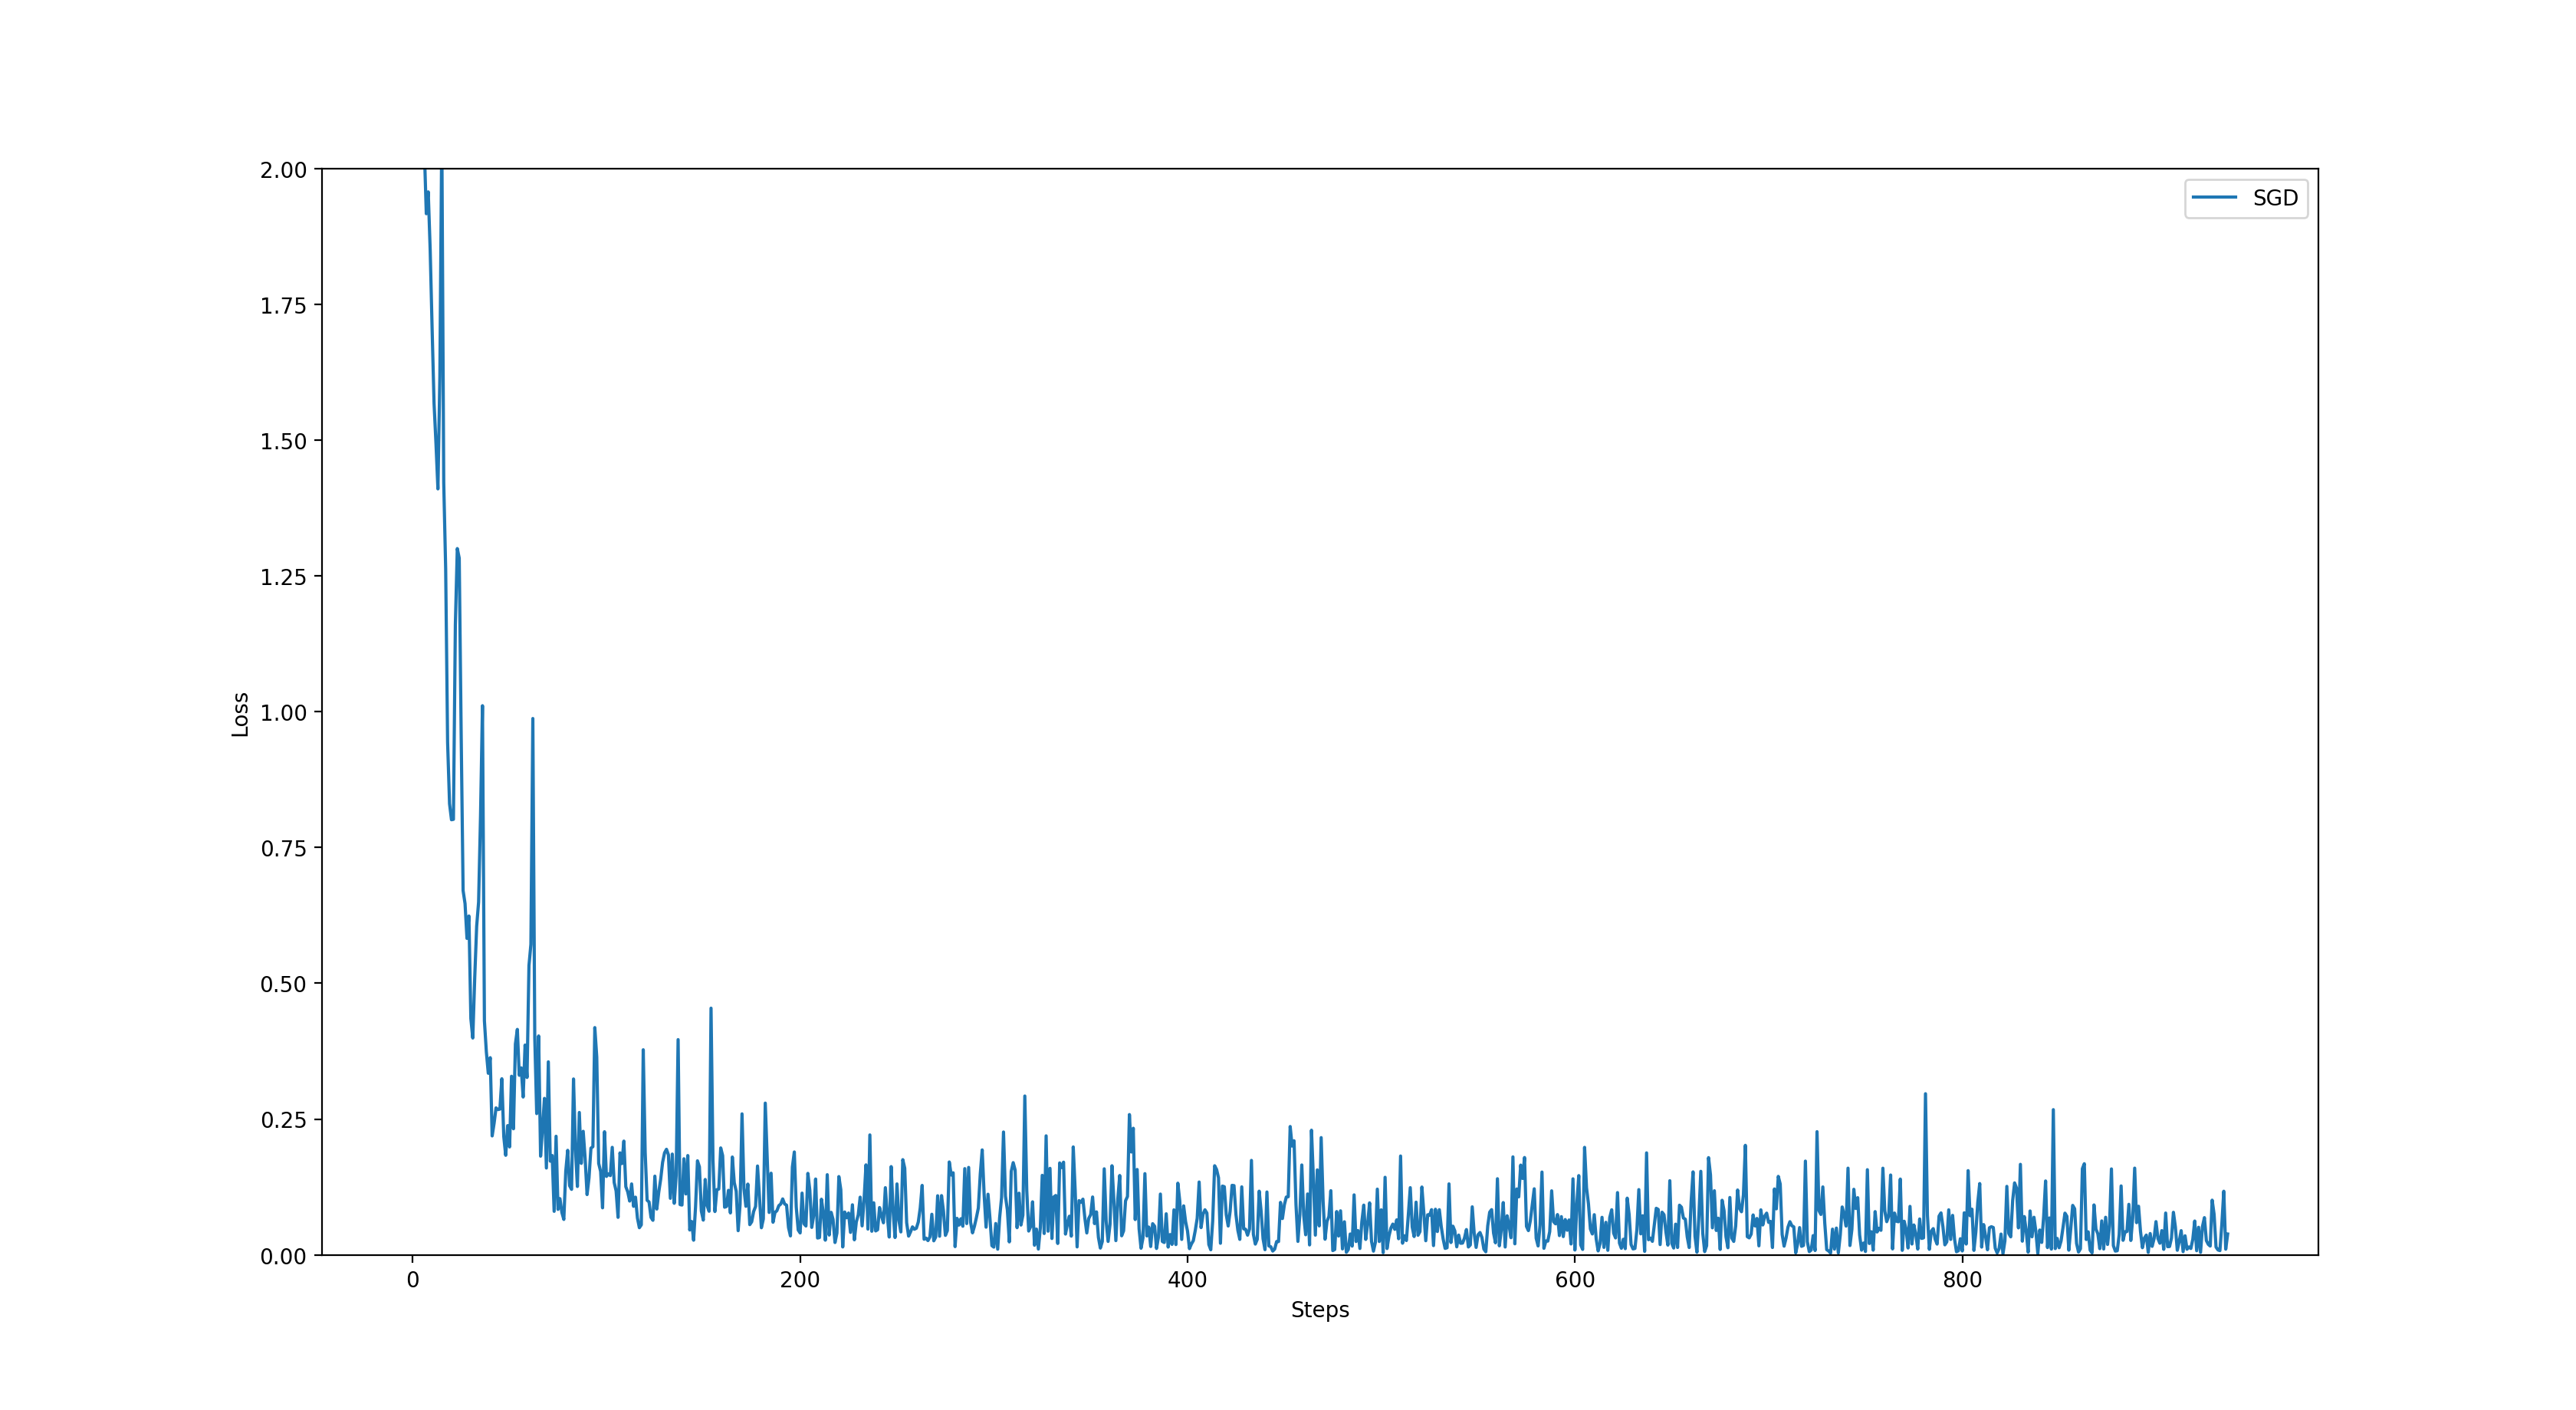
\includegraphics[scale=0.35]{6.png}
                \caption{training loss}
                % \label{fig:pathdemo}
            \end{figure}
            And the validation loss during training is as follows:
            \begin{figure}[H]
                \centering
                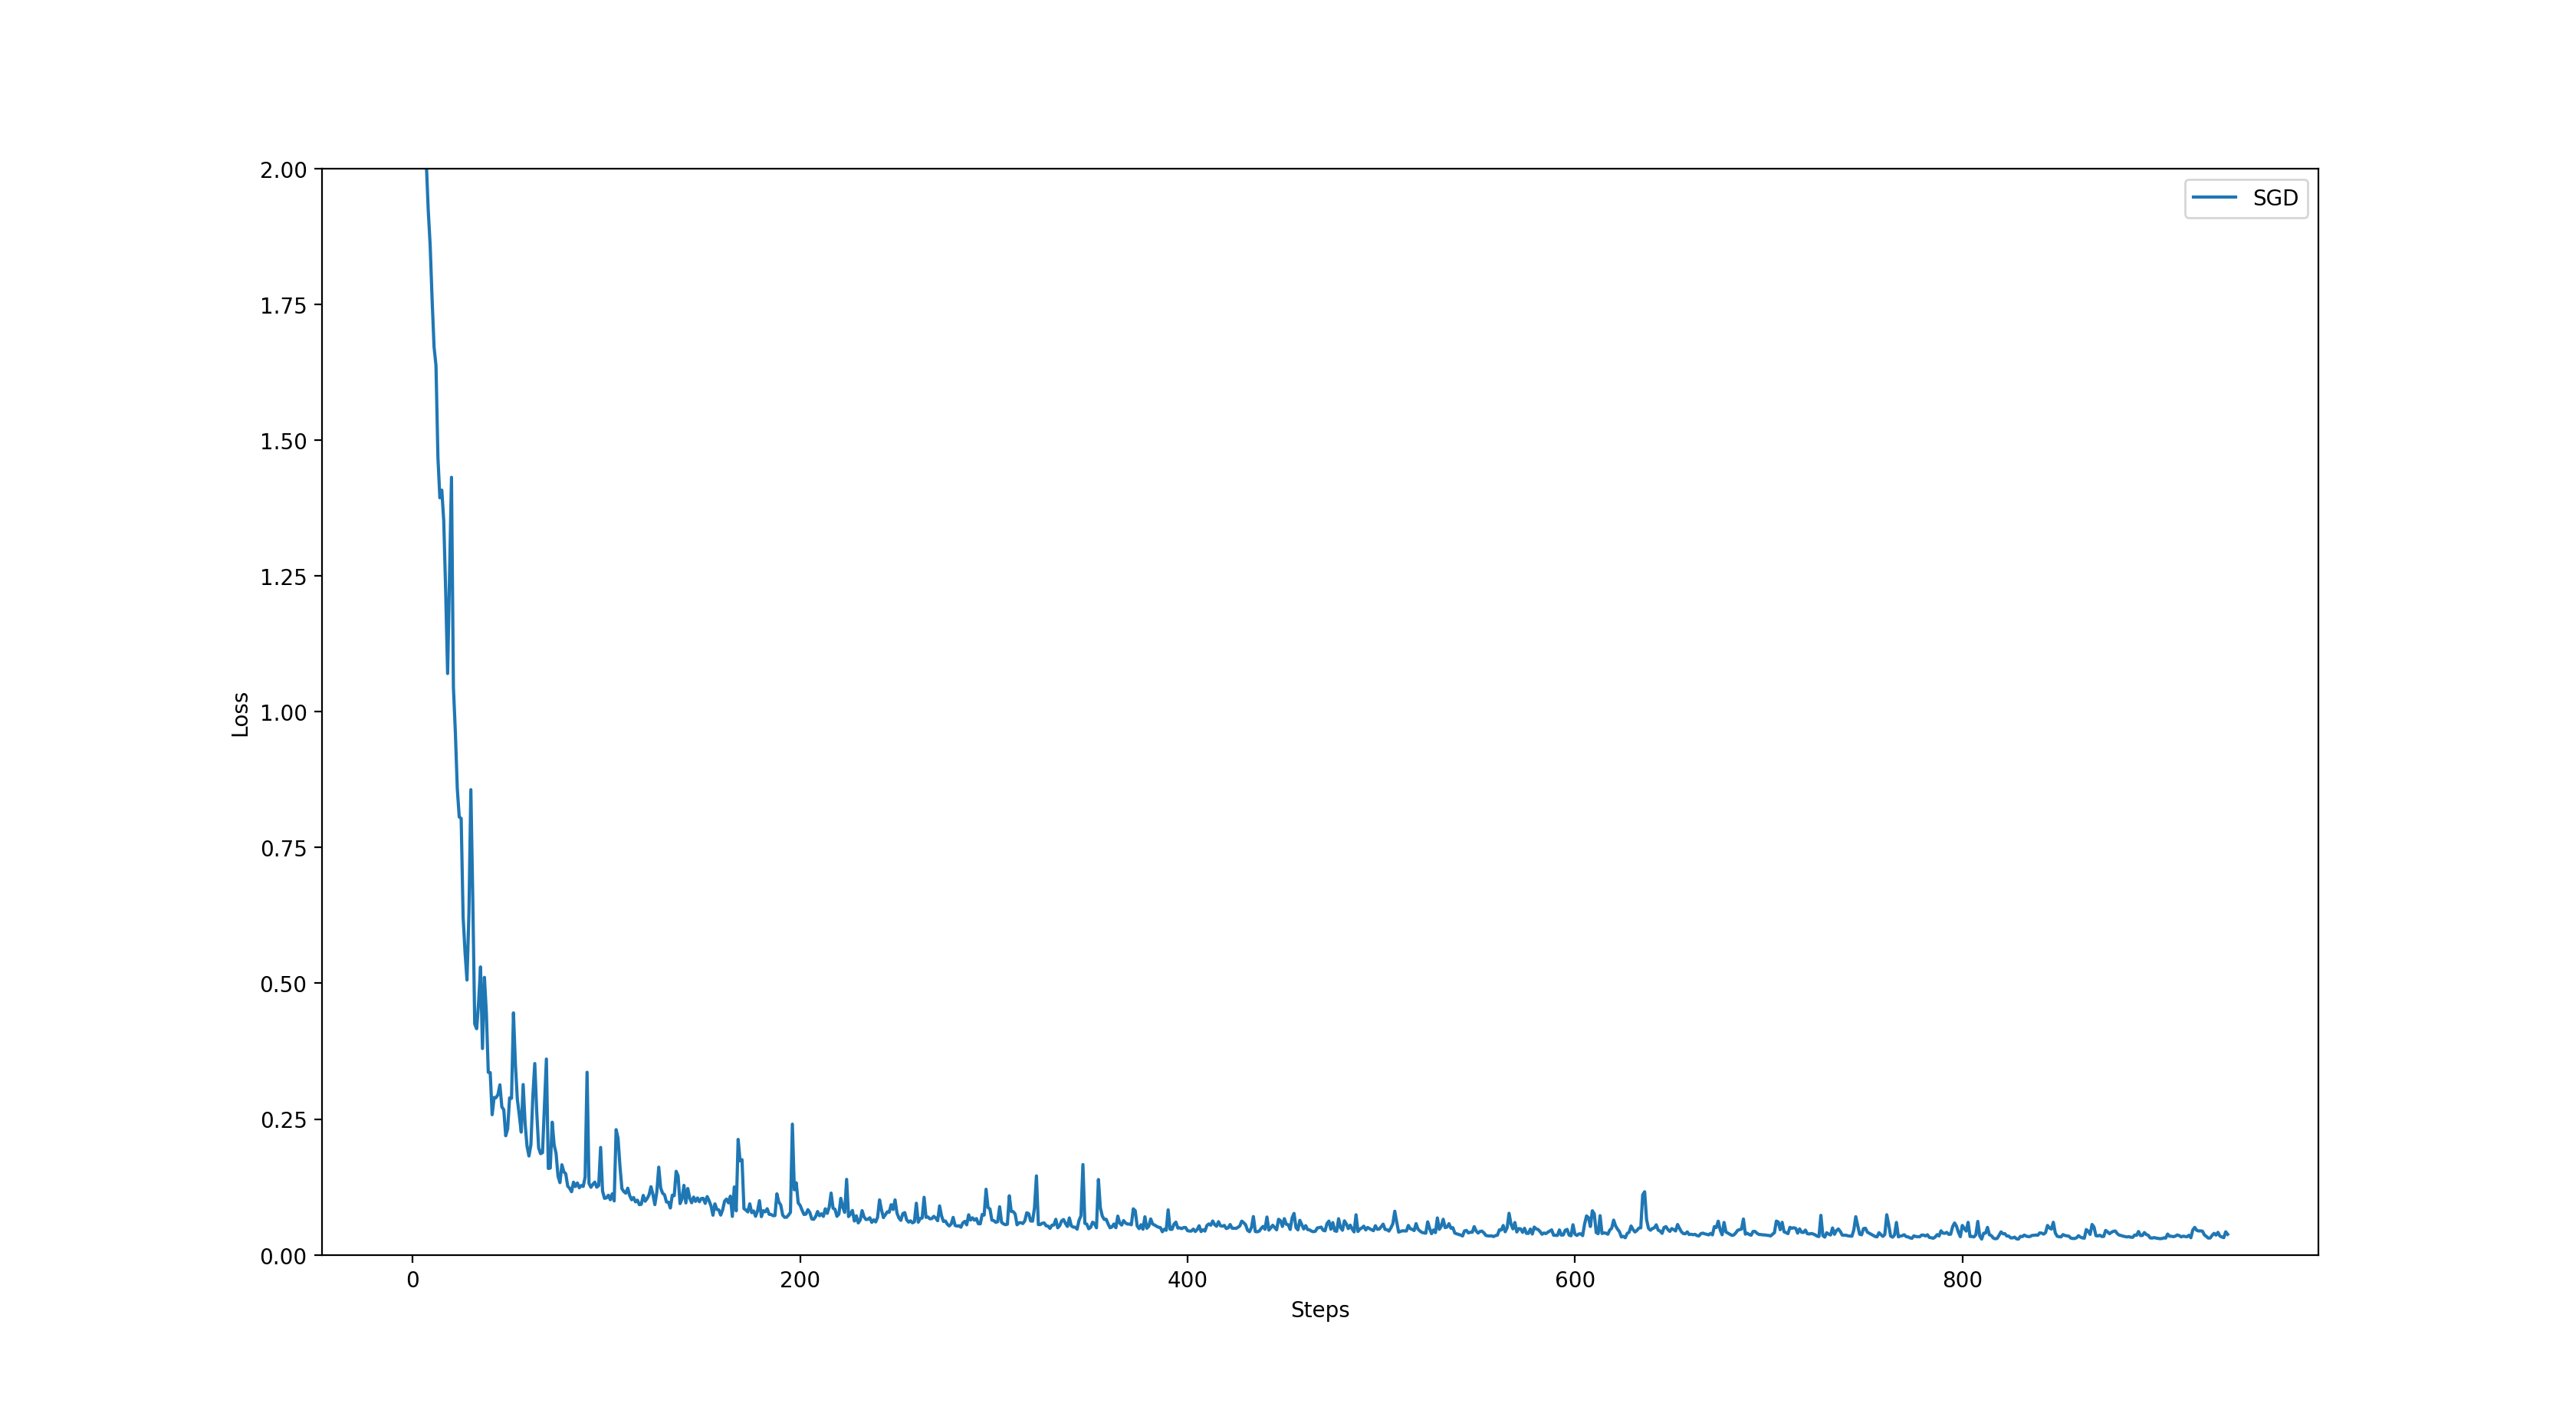
\includegraphics[scale=0.35]{7.png}
                \caption{validation loss}
                % \label{fig:pathdemo}
            \end{figure}
    \end{enumerate}
\end{solution}
%%%%%%%%%%%%%%%%%%%%%
% \begin{problem}[TC 32.3-3]
% \end{problem}

%\begin{remark}

%\end{remark}

% \begin{solution}
%
% \end{solution}
%%%%%%%%%%%%%%%%%%%%
%\newpage
%%%%%%%%%%%%%%%%%%%%


%%%%%%%%%%%%%%%%%%%%%%%%%%%%%%%%%%%%%%%%%%%%%%%%%%%%%%%%%%%%%%%%
%                      Correction START!                       %
%%%%%%%%%%%%%%%%%%%%%%%%%%%%%%%%%%%%%%%%%%%%%%%%%%%%%%%%%%%%%%%%
\begincorrection
%%%%%%%%%%%%%%%%%%%%
%\begin{problem}[]

%\end{problem}

%\begin{cause}
%
%\end{cause}

%\begin{revision}

%\end{revision}
%%%%%%%%%%%%%%%%%%%%
%\newpage
%%%%%%%%%%%%%%%%%%%%


%%%%%%%%%%%%%%%%%%%%%%%%%%%%%%%%%%%%%%%%%%%%%%%%%%%%%%%%%%%%%%%%
%                       Feedback START!                        %
%%%%%%%%%%%%%%%%%%%%%%%%%%%%%%%%%%%%%%%%%%%%%%%%%%%%%%%%%%%%%%%%
\beginfb
%\begin{itemize}
%
%\end{itemize}


%%%%%%%%%%%%%%%%%%%%%%%%%%%%%%%%%%%%%%%%%%%%%%%%%%%%%%%%%%%%%%%%
%                        Homework END!                         %
%%%%%%%%%%%%%%%%%%%%%%%%%%%%%%%%%%%%%%%%%%%%%%%%%%%%%%%%%%%%%%%%
\end{document}

